\chapter{Configuration, Tools, and Platforms}
\label{chap:configuration-tools-platforms}

\section{Database Management System}
The project uses PostgreSQL as its target database management system. This selection is appropriate because PostgreSQL supports both conventional relational database design and the advanced features required by a DBMS-oriented academic project. In the current implementation, the schema and SQL logic rely on several PostgreSQL capabilities, including \texttt{UUID} primary keys, \texttt{JSONB} fields, \texttt{CHECK} constraints, \texttt{GENERATED ALWAYS AS IDENTITY}, \texttt{TIMESTAMPTZ}, and server-side logic implemented through functions, procedures, triggers, and transactions.

The local database environment used for development and testing was verified as PostgreSQL~18.3. This version provides a strong transactional model, expressive SQL syntax, and reliable support for integrity constraints and procedural extensions. These characteristics make PostgreSQL well suited to a project that emphasizes data consistency, business-rule enforcement, and database-side processing for workflows such as enrollment, progress tracking, notifications, and transaction logging.

% Ghi chú tiếng Việt:
% Phần này giải thích vì sao chọn PostgreSQL.
% Điểm nên nhấn mạnh là dự án không chỉ dùng bảng và truy vấn cơ bản,
% mà còn dùng nhiều tính năng nâng cao của PostgreSQL như UUID, JSONB,
% CHECK constraint, trigger, function, procedure và transaction.
% Trong máy hiện tại, phiên bản DB đã kiểm tra được là PostgreSQL 18.3.

\section{Development Environment}
The development environment combines SQL source files, a Flask-based demo application, and supporting tools for editing, testing, and database inspection. According to the repository structure, the database is initialized from \path{ERD.sql}, populated by \path{seed_data.sql}, and extended with procedural logic from \path{procedure_trigger_transaction.sql}. The demonstration layer is implemented in Python and Flask under the \path{demo/} directory, where the application connects directly to PostgreSQL and exposes the main database scenarios through a web interface.

The local machine used for development provides a Windows-based environment with Visual Studio Code for source editing, Git for version control, Python 3.14.4 for runtime execution, Flask 3.1.3 for the demo application, and PostgreSQL 18.3 for data storage and processing. For database interaction, the system also has \texttt{psql} 18.3 and pgAdmin~4 installed, which are appropriate tools for script execution, inspection, and manual verification of the database state.

\begin{figure}[htbp]
    \centering
    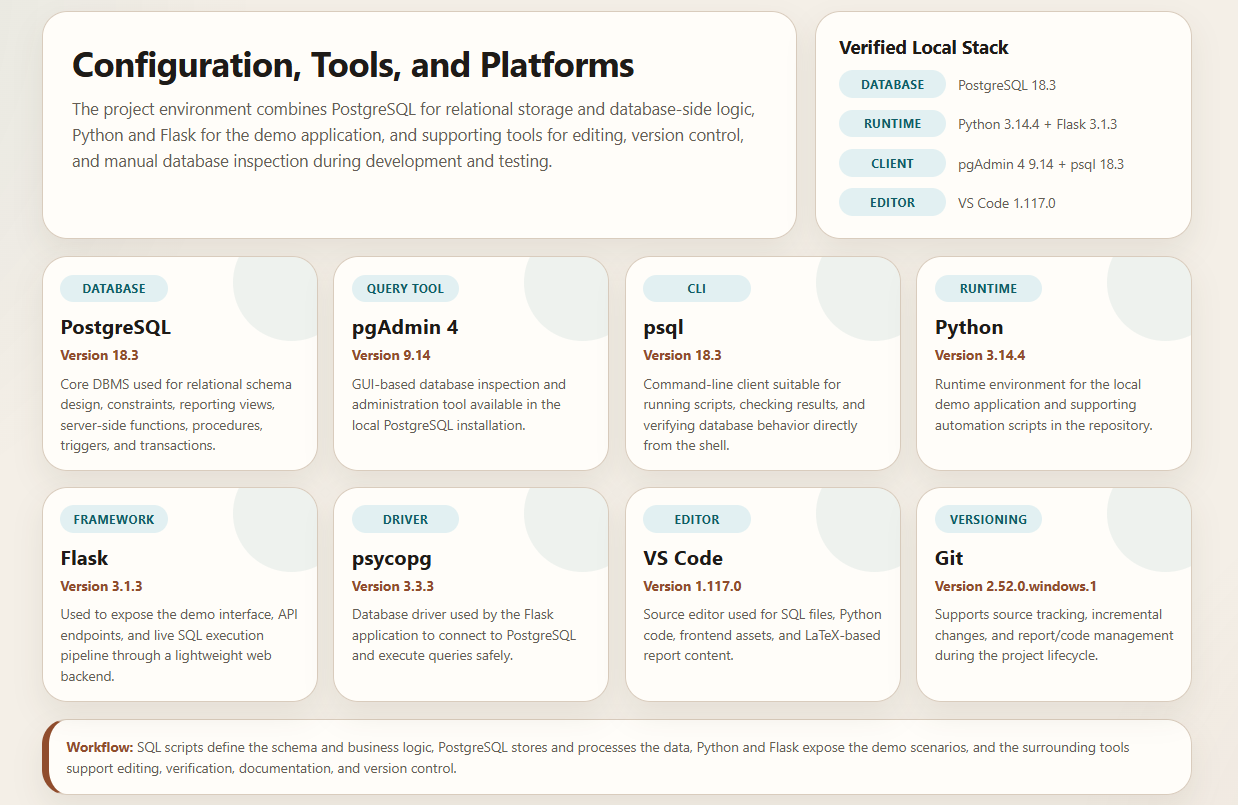
\includegraphics[width=0.96\textwidth]{assets/images/figure_2_1}
    \caption{Development stack and core tools used in the project environment.}
    \label{fig:chapter2-stack}
\end{figure}

% Ghi chú tiếng Việt:
% Phần này mô tả môi trường phát triển thực tế.
% Có thể hiểu đơn giản là:
% SQL scripts -> PostgreSQL -> Flask demo -> browser để trình diễn.
% Đồng thời nêu rõ editor, runtime, Git, và công cụ DB client đang có trên máy.
%
% Ảnh 2.1 đang dùng file figure_2_1.png.
% Nội dung ảnh nên thể hiện stack công nghệ chính của dự án:
% PostgreSQL, pgAdmin/psql, Python, Flask, Git, VS Code và các SQL scripts chính.

\section{Tools and Technologies}
\begin{table}[H]
    \centering
    \small
    \caption{Tools and technologies used in the project}
    \label{tab:tools-technologies}
    \begin{tabular}{p{3.2cm}p{4.2cm}p{6.2cm}}
        \toprule
        \textbf{Category} & \textbf{Tool/Technology} & \textbf{Purpose} \\
        \midrule
        Database & PostgreSQL 18.3 & Relational database implementation, schema definition, constraints, triggers, procedures, functions, and transactions \\
        Query Tool & pgAdmin 4 9.14 / \texttt{psql} 18.3 & Database inspection, script execution, and manual verification of tables and SQL logic \\
        Programming Language & Python 3.14.4 & Runtime environment for the Flask demo application and database connectivity scripts \\
        Web Framework & Flask 3.1.3 & Web backend for the demo interface, API endpoints, and SSE-based progress updates \\
        Database Driver & psycopg 3.3.3 & PostgreSQL connectivity layer used by the Python demo application \\
        Frontend & HTML, CSS, JavaScript & Interactive browser-based interface for demonstrating views, triggers, procedures, and transactions \\
        Source Editor & Visual Studio Code 1.117.0 & Editing SQL files, Python source code, frontend assets, and report files \\
        Documentation & LaTeX / Overleaf & Academic report preparation and final document formatting \\
        Version Control & Git 2.52.0.windows.1 & Source code management and report version tracking \\
        \bottomrule
    \end{tabular}
\end{table}

The technology stack reflects the structure of the project itself. PostgreSQL serves as the central platform for data storage and business logic, while Python and Flask connect the database layer to a demonstrable user-facing interface. The remaining tools support development workflow, editing, version control, and final documentation.

% Ghi chú tiếng Việt:
% Bảng này đã điền sẵn theo công cụ phát hiện được trên máy và trong repo.
% Nếu sau này bạn muốn rút gọn, có thể giữ các hàng quan trọng nhất:
% PostgreSQL, pgAdmin/psql, Python, Flask, Git, VS Code, LaTeX/Overleaf.
% Nếu nhóm có dùng thêm Docker, Postman hoặc draw.io thì có thể thêm một hàng mới.

\section{Hardware Configuration}
The hardware configuration used for development and testing is sufficient for a medium-scale academic database project. The local machine used for this work is equipped with a 13th Gen Intel(R) Core(TM) i5-13420H processor, 15.64~GB of physical memory, and local fixed drives totaling approximately 426.28~GB of storage capacity. At the time of inspection, the machine provided two main fixed drives: a 226.28~GB system drive and a 200.00~GB workspace drive.

The operating environment is a 64-bit Windows platform, identified locally as build 26200 with display version 25H2. This setup is adequate for running PostgreSQL, Python, Flask, the browser-based demo interface, and supporting development tools at the same time. For the scope of the project, the hardware requirements are moderate, but the available CPU, memory, and storage are sufficient for schema creation, data seeding, SQL testing, and interactive demonstration.

\begin{itemize}
    \item CPU: 13th Gen Intel(R) Core(TM) i5-13420H
    \item RAM: 15.64 GB
    \item Storage: 226.28 GB system drive + 200.00 GB workspace drive
    \item Operating System: Windows x64, display version 25H2, build 26200
\end{itemize}

\begin{figure}[htbp]
    \centering
    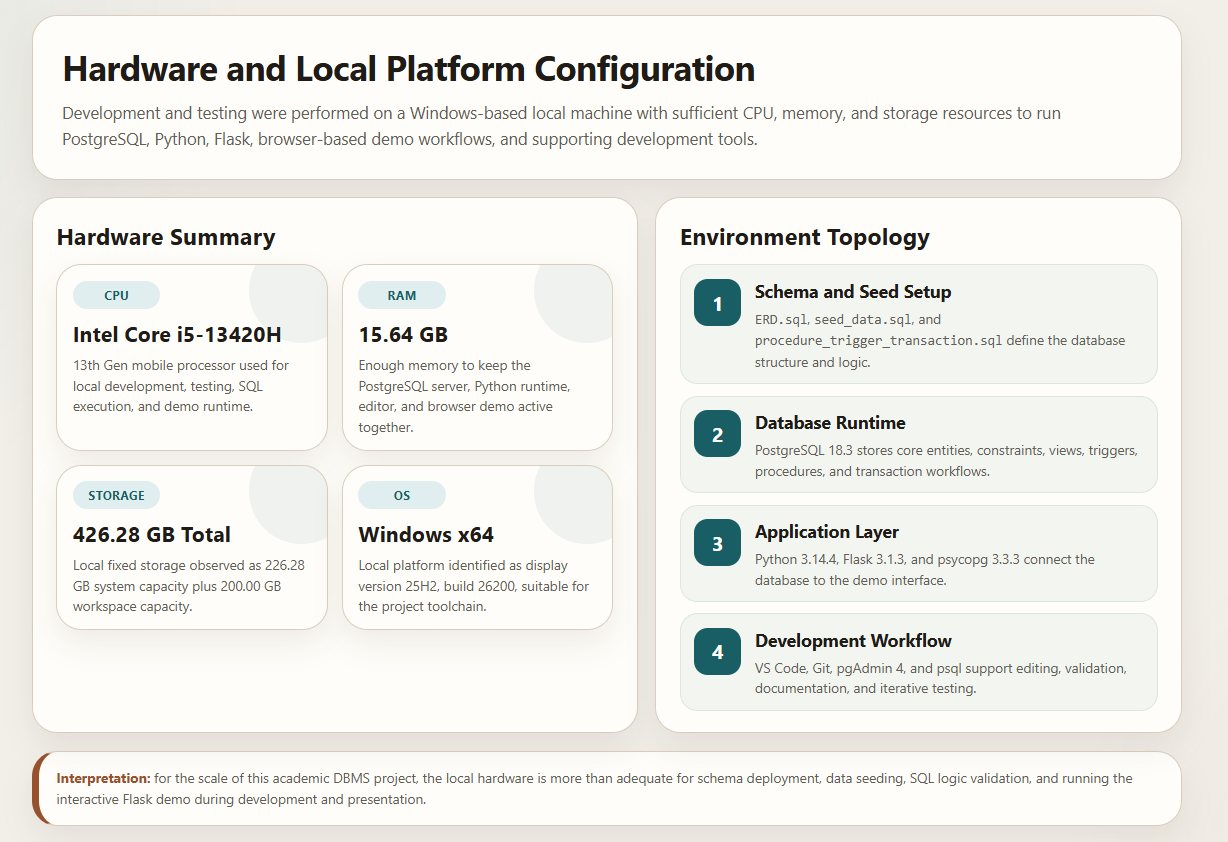
\includegraphics[width=0.96\textwidth]{assets/images/figure_2_2}
    \caption{Hardware and local platform configuration used for development and testing.}
    \label{fig:chapter2-hardware}
\end{figure}

% Ghi chú tiếng Việt:
% Phần này dùng cấu hình máy thật đã kiểm tra được trong môi trường hiện tại.
% Nếu bạn muốn trình bày ngắn hơn, chỉ cần giữ 4 dòng CPU, RAM, Storage, Operating System.
% Nếu sau này chạy demo trên một máy khác, nên sửa lại mục này cho đúng với máy đem đi bảo vệ.
%
% Ảnh 2.2 đang dùng file figure_2_2.png.
% Ảnh này nên minh họa hai ý:
% (1) cấu hình phần cứng và hệ điều hành,
% (2) cách các thành phần môi trường local phối hợp với nhau khi chạy dự án.
